\documentclass[a4paper,12pt]{article} % добавить leqno в [] для нумерации слева
\usepackage[a4paper,top=1.3cm,bottom=2cm,left=1.5cm,right=1.5cm,marginparwidth=0.75cm]{geometry}
%%% Работа с русским языком
\usepackage{cmap}					% поиск в PDF
\usepackage[warn]{mathtext} 		% русские буквы в фомулах
\usepackage[T2A]{fontenc}			% кодировка
\usepackage[utf8]{inputenc}			% кодировка исходного текста
\usepackage[english,russian]{babel}	% локализация и переносы
\usepackage{physics}
\usepackage{multirow}
\usepackage{bm}
\usepackage{longtable}

%%% Нормальное размещение таблиц (писать [H] в окружении таблицы)
\usepackage{float}
\restylefloat{table}


\usepackage{graphicx}

\usepackage{wrapfig}
\usepackage{tabularx}

\usepackage{hyperref}
\usepackage[rgb]{xcolor}
\hypersetup{
	colorlinks=true,urlcolor=blue
}
\usepackage{pgfplots}
\pgfplotsset{compat=1.9}
%%% Дополнительная работа с математикой
\usepackage{amsmath,amsfonts,amssymb,amsthm,mathtools} % AMS
\usepackage{icomma} % "Умная" запятая: $0,2$ --- число, $0, 2$ --- перечисление

%% Номера формул
%\mathtoolsset{showonlyrefs=true} % Показывать номера только у тех формул, на которые есть \eqref{} в тексте,

%% Шрифты
\usepackage{euscript}	 % Шрифт Евклид
\usepackage{mathrsfs} % Красивый матшрифт

%% Свои команды
\DeclareMathOperator{\sgn}{\mathop{sgn}}

%% Перенос знаков в формулах (по Львовскому)
%\newcommand*{\hm}[1]{#1\nobreak\discretionary{}
%	{\hbox{$\mathsurround=0pt #1$}}{}}

\date{\today}

\begin{document}

\begin{titlepage}
	\begin{center}
		{\large МОСКОВСКИЙ ФИЗИКО-ТЕХНИЧЕСКИЙ ИНСТИТУТ (НАЦИОНАЛЬНЫЙ ИССЛЕДОВАТЕЛЬСКИЙ УНИВЕРСИТЕТ)}
	\end{center}
	\begin{center}
		{\large Физтех-школа физики и исследований им. Ландау}
	\end{center}
	
	
	\vspace{4.5cm}
	{\huge
		\begin{center}
			{\bf Отчёт о выполнении лабораторной работы №3.3.4}\\
			Эффект Холла в полупроводниках
		\end{center}
	}
	\vspace{2cm}
	\begin{flushright}
		{\LARGE Автор:\\ Сенокосов Арсений Олегович \\
			\vspace{0.2cm}
			Б02-012}
	\end{flushright}
	\vspace{8cm}
	\begin{center}
		Долгопрудный\\
		\today
	\end{center}
\end{titlepage}
%\numberwithin{equation}{section}

\section{Введение}

\textbf{Цель работы:} измерение подвижности и концентрации носителей заряда в полупроводниках.

\textbf{В работе используются:} электромагнит с источником питания, амперметр, миллиамперметр, милливеберметр, реостат, цифровой вольтметр, источник питания (1.5 В), образцы легированного германия.


\section{Теоретические сведения}

Суть эффекта Холла состоит в следующем. Пусть через однородную пластину металла вдоль оси $ x $ течёт ток $ I $ (рис. \ref{ris1}).

\begin{wrapfigure}{r}{6cm}
	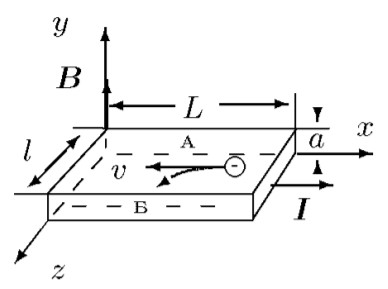
\includegraphics[width=6cm]{holl.jpg}
	\caption{Образец с током в магнитном поле}
	\label{ris1}
\end{wrapfigure}

Если эту пластину поместить в магнитное поле, направленное по оси $ y $, то между гранями А и Б появляется разность потенциалов. В самом деле, на электрон, движущийся со скоростью $ \left\langle \bm{v} \right\rangle $ в электромагнитном поле, действует сила Лоренца:

\[ \bm{F}_\text{л} = -e\bm{E}-e\left\langle\bm{v} \right\rangle\cross\bm{B} \]

где $ e $ -- абсолютная величина заряда электрона, $ \bm{E} $ -- напряжённость электрического поля, $ \bm{B} $ -- индукция магнитного поля. В нашем случае сила, обусловленная вторым слагаемым, направлена вдоль оси $ z $:


\[ F_B = e |\left\langle v_x \right\rangle| B, \]

Здесь $ |\left\langle v_x \right\rangle| $ -- абсолютная величина дрейфовой скорости электронов вдоль оси $ x $, возникающая под действием внешнего электрического поля.

Под действием этой силы электроны отклоняются к грани Б, заряжая её отрицательно (для простоты рассматриваем только один тип носителей). На грани А накапливаются нескомпенсированные положительные заряды. Это приводит к возникновению электрического поля $ E_z $, направленного от А к Б, которое действует на электроны с силой $ F_E=eE_z $, направленной против силы $ F_B $. В установившемся режиме сила $ F_E $ уравновешивает силу $ F_B $, и накопление электрических зарядов на боковых гранях пластины прекращается. Из условия равновесия $ F_B=F_E $ найдём


\[ E_z = |\left\langle v_x \right\rangle| B. \]

Поле $ E_z $ даёт вклад в общее поле $ \bm{E} $, в котором движутся электроны. С полем $ E_z $ связана разность потенциалов $ U_\text{АБ} $ между гранями А и Б:

\[ U_\text{АБ} = -E_z l = - |\left\langle v_x \right\rangle| B l. \]

В этом и состоит эффект Холла. Замечая, что сила тока

\[ I = n e |\left\langle v_x \right\rangle| l a. \]
получаем ЭДС Холла:

\begin{equation}\label{1}
\mathcal{E}_x = U_\text{АБ}= - \frac{IB}{nea} = - R_x \cdot \frac{IB}{a},
\end{equation}

Константа $ R_x $ называется \textit{постоянной Холла}. Как видно из \eqref{1},

\begin{equation}\label{2}
R_x=\frac{1}{ne}.
\end{equation}

\section{Экспериментальная установка}

Электрическая схема установки для измерения ЭДС Холла представлена на рис. \ref{ust}. В зазоре электромагнита (рис. \ref{ust}а) создаётся постоянное магнитное поле, величину которого можно менять с помощью регулятора $ R_1 $ источника питания электромагнита. Ток питания электромагнита измеряется амперметром $ A_1 $ Разъём $ K_1 $ позволяет менять направление тока в обмотках электромагнита. Градуировка магнита проводится при помощи милливеберметра.

Образец из легированного германия, смонтированный в специальном держателе (рис. \ref{ust}б). подключается к источнику питания ($ \approx 1.5 $ В).

При замыкании ключа $ K_2 $ вдоль длинной стороны образца течёт ток, величина которого регулируется реостатом $ R_2 $ и измеряется миллиамперметром $ A_2 $.


В образце с током, помещённом в зазор электромагнита, между контактами 3 и 4 возникает разность потенциалов $ U_{34} $, которая измеряется с помощью цифрового вольтметра.

\begin{figure}[h]
	\centering
	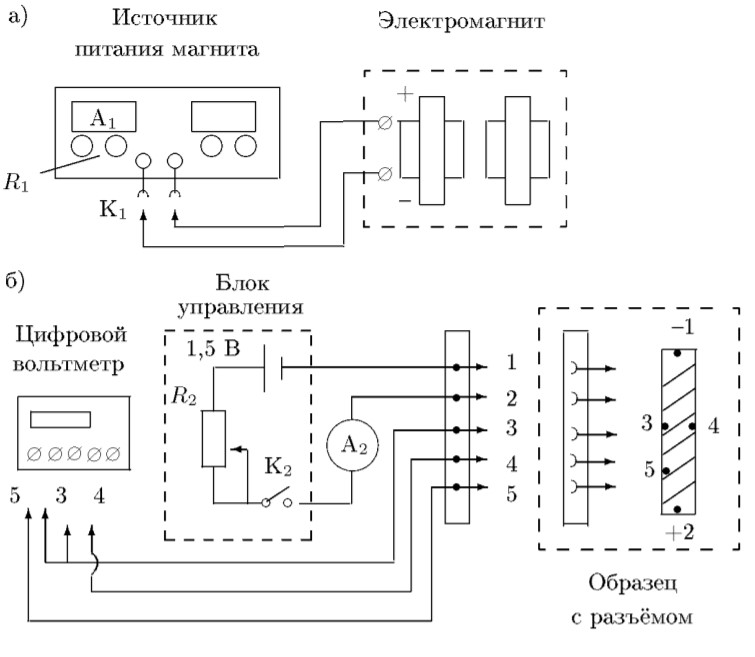
\includegraphics[width=15cm]{ust.jpg}
	\caption{Схема установки для исследования эффекта Холла	в полупроводниках}
	\label{ust}
\end{figure}

Иногда контакты 3 и 4 вследствие неточности подпайки не лежат на одной эквипотенциали, и тогда напряжение между ними связано не только с эффектом Холла, но и с омическим падением напряжения, вызванным протеканием основного тока через образец. Измеряемая разность потенциалов при одном направлении магнитного поля равна сумме ЭДС Холла и омического падения напряжения, а при другом — их разности. В этом случае ЭДС Холла $ \mathcal{E}_x $ может быть определена как половина алгебраической разности показаний вольтметра, полученных для двух противоположных направлений магнитного поля в зазоре. Знак измеряемого напряжения высвечивается на цифровом табло вольтметра.

Можно исключить влияние омического падения напряжения иначе, если при каждом токе через образец измерять напряжение между точками 3 и 4 в отсутствие магнитного поля. При фиксированном токе через образец это дополнительное к ЭДС Холла напряжение $ U_0 $ остаётся неизменным. От него следует (с учётом знака) отсчитывать величину ЭДС Холла:

\begin{equation}\label{3}
\mathcal{E}_x = U_{34} \pm U_0.
\end{equation}

При таком способе измерения нет необходимости проводить повторные измерения с противоположным направлением магнитного поля.

По знаку $ \mathcal{E} $ можно определить характер проводимости -- электронный или дырочный. Для этого необходимо знать направление тока в образце и направление магнитного поля.

Измерив ток $ I $ в образце и напряжение $ U_{35} $ между контактами 3 и 5 в отсутствие магнитного поля, можно, зная параметры образца, рассчитать проводимость материала образца по формуле

\begin{equation}\label{4}
\sigma = \frac{IL_{35}}{U_{35}al},
\end{equation}

где $ L_{35} $ -- расстояние между контактами 3 и 5, $ a $ -- толщина образца, $ l $ -- его ширина.

\section{Ход работы}

\subsection{Градуировка электромагнита}

При помощи тесламетра установим зависимость величины магнитной индукции между полюсами прибора от тока в катушках электромагнита. Результаты измерений занесём в таблицу \ref{tab1}.

\begin{table}[H]
	\centering
	\begin{tabular}{|c|c|c|c|}
		\hline
		$ I_\text{м} $, А & $ B $, мТл & $ I_\text{м} $, А & $ B $, мТл  \\ \hline
		0,10  & 112,1 & 0,80  & 801,1  \\ \hline
		0,20  & 202,9 & 0,90  & 870,5  \\ \hline
		0,30  & 318,2 & 1,00  & 914,3  \\ \hline
		0,40  & 428,1 & 1,10  & 951,8  \\ \hline
		0,50  & 525,4 & 1,20  & 992,3  \\ \hline
		0,60  & 632,3 & 1,33  & 1031,6 \\ \hline
		0,70  & 719,3 & 1,40  & 1048,6 \\ \hline
	\end{tabular}
	\caption{Градуировка электромагнита}
	\label{tab1}
\end{table}

По полученным данным построим график зависимости $ B=f(I_\text{м}) $,

\begin{center}
	\begin{tikzpicture}
	\begin{axis}[
	title={График 1 \quad График зависимости $ B(I_\text{м}) $},
	xlabel={$ I_\text{м} $, А},
	ylabel={$ B $, мТл},
	legend pos=north west,
	xmajorgrids=true,
	ymajorgrids=true,
	grid style=dashed,
	width = 520,
	height = 210,
	%xmin = 300,
	%xmax = 335,
	%ymin =40,
	%ymax =135,
	]
	\legend{ 
		Экспериментальные данные,
	};
	\addplot+ [blue, only marks, mark size = 4pt,
	error bars/.cd,
	x dir=both, x explicit,
	y dir=both, y explicit, 
	] table [x = T, y = sigma,] {
		T	sigma               
		0.10	112.1
		0.20	202.9
		0.30	318.2
		0.40	428.1
		0.50	525.4
		0.60	632.3
		0.70	719.3
		0.80	801.1
		0.90	870.5
		1.00	914.3
		1.10	951.8
		1.20	992.3
		1.33	1031.6
		1.40	1048.6
		1.44	1072.6
	};
%	\addplot [red, domain=297:350, line width =3,2pt] {108,6  -0,155*x};
	\end{axis}
	\end{tikzpicture}
\end{center}


\subsection{Измерение ЭДС Холла}

Для разных значений $ I $ через образец снимем зависимость ЭДС Холла от тока $ I_\text{м} $ через электромагнит. Результаты измерений занесём в таблицу \ref{tab2}.

\begin{table}[H]
	\centering
	\begin{tabular}{l|cc|cc|cc|}
		\hline
		\multicolumn{1}{|c|}{$I$, мА}   & \multicolumn{2}{c|}{0,15}                      & \multicolumn{2}{c|}{0,30}                      & \multicolumn{2}{c|}{0,40}                      \\ \hline
		\multicolumn{1}{|c|}{$U_0$, мВ} & \multicolumn{2}{c|}{-0,023}                    & \multicolumn{2}{c|}{-0,056}                    & \multicolumn{2}{c|}{-0,074}                    \\ \hline
		\multicolumn{1}{c|}{}           & \multicolumn{1}{c|}{$I_\text{м}$, А} & $U$, мВ & \multicolumn{1}{c|}{$I_\text{м}$, А} & $U$, мВ & \multicolumn{1}{c|}{$I_\text{м}$, А} & $U$, мВ \\ \cline{2-7} 
		\multicolumn{1}{c|}{}           & \multicolumn{1}{c|}{0,20}            & -0,051  & \multicolumn{1}{c|}{0,20}            & -0,116  & \multicolumn{1}{c|}{0,20}            & -0,158  \\ \cline{2-7} 
		\multicolumn{1}{c|}{}           & \multicolumn{1}{c|}{0,40}            & -0,081  & \multicolumn{1}{c|}{0,40}            & -0,174  & \multicolumn{1}{c|}{0,40}            & -0,232  \\ \cline{2-7} 
		\multicolumn{1}{c|}{}           & \multicolumn{1}{c|}{0,60}            & -0,106  & \multicolumn{1}{c|}{0,60}            & -0,231  & \multicolumn{1}{c|}{0,60}            & -0,310  \\ \cline{2-7} 
		\multicolumn{1}{c|}{}           & \multicolumn{1}{c|}{0,80}            & -0,130  & \multicolumn{1}{c|}{0,80}            & -0,277  & \multicolumn{1}{c|}{0,80}            & -0,371  \\ \cline{2-7} 
		\multicolumn{1}{c|}{}           & \multicolumn{1}{c|}{1,00}            & -0,146  & \multicolumn{1}{c|}{1,00}            & -0,310  & \multicolumn{1}{c|}{1,00}            & -0,416  \\ \cline{2-7} 
		\multicolumn{1}{c|}{}           & \multicolumn{1}{c|}{1,20}            & -0,156  & \multicolumn{1}{c|}{1,20}            & -0,332  & \multicolumn{1}{c|}{1,20}            & -0,446  \\ \cline{2-7} 
		\multicolumn{1}{c|}{}           & \multicolumn{1}{c|}{1,40}            & -0,164  & \multicolumn{1}{c|}{1,40}            & -0,350  & \multicolumn{1}{c|}{1,40}            & -0,471  \\ \hline
		\multicolumn{1}{|c|}{$I$, мА}   & \multicolumn{2}{c|}{0,50}                      & \multicolumn{2}{c|}{0,60}                      & \multicolumn{2}{c|}{0,70}                      \\ \hline
		\multicolumn{1}{|c|}{$U_0$, мВ} & \multicolumn{2}{c|}{-0,094}                    & \multicolumn{2}{c|}{-0,114}                    & \multicolumn{2}{c|}{-0,134}                    \\ \hline
		& \multicolumn{1}{c|}{$I_\text{м}$, А} & $U$, мВ & \multicolumn{1}{c|}{$I_\text{м}$, А} & $U$, мВ & \multicolumn{1}{c|}{$I_\text{м}$, А} & $U$, мВ \\ \cline{2-7} 
		& \multicolumn{1}{c|}{0,20}            & -0,200  & \multicolumn{1}{c|}{0,20}            & -0,238  & \multicolumn{1}{c|}{0,20}            & -0,281  \\ \cline{2-7} 
		& \multicolumn{1}{c|}{0,40}            & -0,295  & \multicolumn{1}{c|}{0,40}            & -0,354  & \multicolumn{1}{c|}{0,40}            & -0,419  \\ \cline{2-7} 
		& \multicolumn{1}{c|}{0,60}            & -0,381  & \multicolumn{1}{c|}{0,60}            & -0,465  & \multicolumn{1}{c|}{0,60}            & -0,543  \\ \cline{2-7} 
		& \multicolumn{1}{c|}{0,80}            & -0,463  & \multicolumn{1}{c|}{0,80}            & -0,562  & \multicolumn{1}{c|}{0,80}            & -0,656  \\ \cline{2-7} 
		& \multicolumn{1}{c|}{1,00}            & -0,520  & \multicolumn{1}{c|}{1,00}            & -0,629  & \multicolumn{1}{c|}{1,00}            & -0,736  \\ \cline{2-7} 
		& \multicolumn{1}{c|}{1,20}            & -0,560  & \multicolumn{1}{c|}{1,20}            & -0,677  & \multicolumn{1}{c|}{1,20}            & -0,792  \\ \cline{2-7} 
		& \multicolumn{1}{c|}{1,40}            & -0,587  & \multicolumn{1}{c|}{1,40}            & -0,711  & \multicolumn{1}{c|}{1,40}            & -0,832  \\ \hline
		\multicolumn{1}{|c|}{$I$, мА}   & \multicolumn{2}{c|}{0,80}                      & \multicolumn{2}{c|}{1,00}                      & \multicolumn{2}{c|}{1,00 (flip)}                      \\ \hline
		\multicolumn{1}{|c|}{$U_0$, мВ} & \multicolumn{2}{c|}{-0,155}                    & \multicolumn{2}{c|}{-0,194}                    & \multicolumn{2}{c|}{-0,194 (flip)}                    \\ \hline
		& \multicolumn{1}{c|}{$I_\text{м}$, А} & $U$, мВ & \multicolumn{1}{c|}{$I_\text{м}$, А} & $U$, мВ & \multicolumn{1}{c|}{$I_\text{м}$, А} & $U$, мВ \\ \cline{2-7} 
		& \multicolumn{1}{c|}{0,20}            & -0,317  & \multicolumn{1}{c|}{0,20}            & -0,401  & \multicolumn{1}{c|}{0,20}            & 0,004   \\ \cline{2-7} 
		& \multicolumn{1}{c|}{0,40}            & -0,480  & \multicolumn{1}{c|}{0,40}            & -0,562  & \multicolumn{1}{c|}{0,40}            & 0,210   \\ \cline{2-7} 
		& \multicolumn{1}{c|}{0,60}            & -0,625  & \multicolumn{1}{c|}{0,60}            & -0,779  & \multicolumn{1}{c|}{0,60}            & 0,392   \\ \cline{2-7} 
		& \multicolumn{1}{c|}{0,80}            & -0,751  & \multicolumn{1}{c|}{0,80}            & -0,938  & \multicolumn{1}{c|}{0,80}            & 0,549   \\ \cline{2-7} 
		& \multicolumn{1}{c|}{1,00}            & -0,842  & \multicolumn{1}{c|}{1,00}            & -1,044  & \multicolumn{1}{c|}{1,00}            & 0,663   \\ \cline{2-7} 
		& \multicolumn{1}{c|}{1,20}            & -0,906  & \multicolumn{1}{c|}{1,20}            & -1,135  & \multicolumn{1}{c|}{1,20}            & 0,748   \\ \cline{2-7} 
		& \multicolumn{1}{c|}{1,40}            & -0,953  & \multicolumn{1}{c|}{1,40}            & -1,191  & \multicolumn{1}{c|}{1,40}            & 0,797   \\ \cline{2-7} 
	\end{tabular}
	\caption{Измерение ЭДС Холла}
	\label{tab2}
\end{table}

Последнее измерение было произведено при изменённой ориентации образца. Теперь вычислим значение $ \mathcal{E}_x $ по разности показаний вольтметра и сопоставим токи в электромагните с соответствующими значениями индукции магнитного поля. Полученные результаты занесём в таблицу \ref{tab3}.

% Please add the following required packages to your document preamble:
% \usepackage{longtable}
% Note: It may be necessary to compile the document several times to get a multi-page table to line up properly
\begin{longtable}[c]{c|cc|cc|cc|}
	\hline
	\multicolumn{1}{|c|}{$I$, мА} & \multicolumn{2}{c|}{0,15}                          & \multicolumn{2}{c|}{0,30}                          & \multicolumn{2}{c|}{0,40}                          \\ \hline
	\endfirsthead
	%
	\endhead
	%
	& \multicolumn{1}{c|}{$B$, мТл} & $\mathcal{E}_x$, мВ & \multicolumn{1}{c|}{$B$, мТл} & $\mathcal{E}_x$, мВ & \multicolumn{1}{c|}{$B$, мТл} & $\mathcal{E}_x$, мВ \\ \cline{2-7} 
	& \multicolumn{1}{c|}{202,9}   & 0,028               & \multicolumn{1}{c|}{202,9}   & 0,060               & \multicolumn{1}{c|}{202,9}   & 0,084               \\ \cline{2-7} 
	& \multicolumn{1}{c|}{428,1}   & 0,058               & \multicolumn{1}{c|}{428,1}   & 0,118               & \multicolumn{1}{c|}{428,1}   & 0,158               \\ \cline{2-7} 
	& \multicolumn{1}{c|}{632,3}   & 0,083               & \multicolumn{1}{c|}{632,3}   & 0,175               & \multicolumn{1}{c|}{632,3}   & 0,236               \\ \cline{2-7} 
	& \multicolumn{1}{c|}{801,1}   & 0,107               & \multicolumn{1}{c|}{801,1}   & 0,221               & \multicolumn{1}{c|}{801,1}   & 0,297               \\ \cline{2-7} 
	& \multicolumn{1}{c|}{914,3}   & 0,123               & \multicolumn{1}{c|}{914,3}   & 0,254               & \multicolumn{1}{c|}{914,3}   & 0,342               \\ \cline{2-7} 
	& \multicolumn{1}{c|}{992,3}   & 0,133               & \multicolumn{1}{c|}{992,3}   & 0,276               & \multicolumn{1}{c|}{992,3}   & 0,372               \\ \cline{2-7} 
	& \multicolumn{1}{c|}{1048,6}  & 0,141               & \multicolumn{1}{c|}{1048,6}  & 0,294               & \multicolumn{1}{c|}{1048,6}  & 0,397               \\ \hline
	\multicolumn{1}{|c|}{$I$, мА} & \multicolumn{2}{c|}{0,50}                          & \multicolumn{2}{c|}{0,60}                          & \multicolumn{2}{c|}{0,70}                          \\ \hline
	& \multicolumn{1}{c|}{$B$, мТл} & $\mathcal{E}_x$, мВ & \multicolumn{1}{c|}{$B$, мТл} & $\mathcal{E}_x$, мВ & \multicolumn{1}{c|}{$B$, мТл} & $\mathcal{E}_x$, мВ \\ \cline{2-7} 
	& \multicolumn{1}{c|}{202,9}   & 0,106               & \multicolumn{1}{c|}{202,9}   & 0,124               & \multicolumn{1}{c|}{202,9}   & 0,147               \\ \cline{2-7} 
	& \multicolumn{1}{c|}{428,1}   & 0,201               & \multicolumn{1}{c|}{428,1}   & 0,240               & \multicolumn{1}{c|}{428,1}   & 0,285               \\ \cline{2-7} 
	& \multicolumn{1}{c|}{632,3}   & 0,287               & \multicolumn{1}{c|}{632,3}   & 0,351               & \multicolumn{1}{c|}{632,3}   & 0,409               \\ \cline{2-7} 
	& \multicolumn{1}{c|}{801,1}   & 0,369               & \multicolumn{1}{c|}{801,1}   & 0,448               & \multicolumn{1}{c|}{801,1}   & 0,522               \\ \cline{2-7} 
	& \multicolumn{1}{c|}{914,3}   & 0,426               & \multicolumn{1}{c|}{914,3}   & 0,515               & \multicolumn{1}{c|}{914,3}   & 0,602               \\ \cline{2-7} 
	& \multicolumn{1}{c|}{992,3}   & 0,466               & \multicolumn{1}{c|}{992,3}   & 0,563               & \multicolumn{1}{c|}{992,3}   & 0,658               \\ \cline{2-7} 
	& \multicolumn{1}{c|}{1048,6}  & 0,493               & \multicolumn{1}{c|}{1048,6}  & 0,597               & \multicolumn{1}{c|}{1048,6}  & 0,698               \\ \hline
	\multicolumn{1}{|c|}{$I$, мА} & \multicolumn{2}{c|}{0,80}                          & \multicolumn{2}{c|}{1,00}                          & \multicolumn{2}{c|}{1,00 (flipped)}                \\ \hline
	& \multicolumn{1}{c|}{$B$, мТл} & $\mathcal{E}_x$, мВ & \multicolumn{1}{c|}{$B$, мТл} & $\mathcal{E}_x$, мВ & \multicolumn{1}{c|}{$B$, мТл} & $\mathcal{E}_x$, мВ \\ \cline{2-7} 
	& \multicolumn{1}{c|}{202,9}   & 0,162               & \multicolumn{1}{c|}{202,9}   & 0,207               & \multicolumn{1}{c|}{202,9}   & 0,198               \\ \cline{2-7} 
	& \multicolumn{1}{c|}{428,1}   & 0,325               & \multicolumn{1}{c|}{428,1}   & 0,368               & \multicolumn{1}{c|}{428,1}   & 0,404               \\ \cline{2-7} 
	& \multicolumn{1}{c|}{632,3}   & 0,470               & \multicolumn{1}{c|}{632,3}   & 0,585               & \multicolumn{1}{c|}{632,3}   & 0,586               \\ \cline{2-7} 
	& \multicolumn{1}{c|}{801,1}   & 0,596               & \multicolumn{1}{c|}{801,1}   & 0,744               & \multicolumn{1}{c|}{801,1}   & 0,743               \\ \cline{2-7} 
	& \multicolumn{1}{c|}{914,3}   & 0,687               & \multicolumn{1}{c|}{914,3}   & 0,850               & \multicolumn{1}{c|}{914,3}   & 0,857               \\ \cline{2-7} 
	& \multicolumn{1}{c|}{992,3}   & 0,751               & \multicolumn{1}{c|}{992,3}   & 0,941               & \multicolumn{1}{c|}{992,3}   & 0,942               \\ \cline{2-7} 
	& \multicolumn{1}{c|}{1048,6}  & 0,798               & \multicolumn{1}{c|}{1048,6}  & 0,997               & \multicolumn{1}{c|}{1048,6}  & 0,991               \\ \cline{2-7} 
	\caption{Результаты вычислений}
	\label{tab3}\\
\end{longtable}

По полученным данным построим графики зависимости $ \mathcal{E}_x(B) $ для различных значений $ I $.


\begin{center}
	\begin{tikzpicture}
	\begin{axis}[
	title={График 2 \quad Графики зависимости $ \mathcal{E}_x(B) $},
	xlabel={$ B $, мТлл},
	ylabel={$ \mathcal{E}_x $, мВ},
	legend pos=north west,
	xmajorgrids=true,
	ymajorgrids=true,
	grid style=dashed,
	width = 520,
	height = 380,
	%xmin = 300,
	%xmax = 335,
	%ymin =40,
	%ymax =135,
	]
	\legend{
	$ I_\text{м}  = 0.15 $ мА,
	$ I_\text{м}  = 0.30 $ мА,
	$ I_\text{м}  = 0.40 $ мА,
	$ I_\text{м}  = 0.50 $ мА,
	$ I_\text{м}  = 0.60 $ мА,
	$ I_\text{м}  = 0.70 $ мА,
	$ I_\text{м}  = 0.80 $ мА,
	$ I_\text{м}  = 1.00 $ мА,
	$ I^{flip}_\text{м}  = 1.00 $ мА,,,,,,,,,};
	\addplot+ [ only marks, mark size = 4pt, mark=*,
	error bars/.cd,
	x dir=both, x explicit,
	y dir=both, y explicit, 
	] table [x = T, y = sigma,] {
		T	sigma               
		202.9	0.028
		428.1	0.058
		632.3	0.083
		801.1	0.107
		914.3	0.123
		992.3	0.133
		1048.6	0.141
	};
	\addplot+ [ only marks, mark size = 4pt, mark=oplus*,
	error bars/.cd,
	x dir=both, x explicit,
	y dir=both, y explicit, 
	] table [x = T, y = sigma,] {
		T	sigma               
		202.9	0.060
		428.1	0.118
		632.3	0.175
		801.1	0.221
		914.3	0.254
		992.3	0.276
		1048.6	0.294
	};
	\addplot+ [ only marks, mark size = 4pt, mark=square*,
	error bars/.cd,
	x dir=both, x explicit,
	y dir=both, y explicit, 
	] table [x = T, y = sigma,] {
		T	sigma               
		202.9	0.084
		428.1	0.158
		632.3	0.236
		801.1	0.297
		914.3	0.342
		992.3	0.372
		1048.6	0.397	
	};
	\addplot+ [ only marks, mark size = 4pt, mark=triangle*,
	error bars/.cd,
	x dir=both, x explicit,
	y dir=both, y explicit, 
	] table [x = T, y = sigma,] {
		T	sigma               
		202.9	0.106
		428.1	0.201
		632.3	0.287
		801.1	0.369
		914.3	0.426
		992.3	0.466
		1048.6	0.493	
	};
	\addplot+ [ only marks, mark size = 4pt, mark=diamond*,
	error bars/.cd,
	x dir=both, x explicit,
	y dir=both, y explicit, 
	] table [x = T, y = sigma,] {
		T	sigma               
		202.9	0.124
		428.1	0.240
		632.3	0.351
		801.1	0.448
		914.3	0.515
		992.3	0.563
		1048.6	0.597	
	};
	\addplot+ [ only marks, mark size = 4pt, mark=halfdiamond*,
	error bars/.cd,
	x dir=both, x explicit,
	y dir=both, y explicit, 
	] table [x = T, y = sigma,] {
		T	sigma               
		202.9	0.147
		428.1	0.285
		632.3	0.409
		801.1	0.522
		914.3	0.602
		992.3	0.658
		1048.6	0.698	
	};
	\addplot+ [ only marks, mark size = 4pt, mark=halfsquare right*,
	error bars/.cd,
	x dir=both, x explicit,
	y dir=both, y explicit, 
	] table [x = T, y = sigma,] {
		T	sigma               
		202.9	0.162
		428.1	0.325
		632.3	0.470
		801.1	0.596
		914.3	0.687
		992.3	0.751
		1048.6	0.798	
	};
	\addplot+ [ only marks, mark size = 4pt, mark=pentagon*,
	error bars/.cd,
	x dir=both, x explicit,
	y dir=both, y explicit, 
	] table [x = T, y = sigma,] {
		T	sigma               
		202.9	0.207
		428.1	0.368
		632.3	0.585
		801.1	0.744
		914.3	0.850
		992.3	0.941
		1048.6	0.997
	};
	\addplot+ [ only marks, mark size = 4pt, mark=halfsquare left*,
	error bars/.cd,
	x dir=both, x explicit,
	y dir=both, y explicit, 
	] table [x = T, y = sigma,] {
		T	sigma               
		202.9	0.198
		428.1	0.404
		632.3	0.586
		801.1	0.743
		914.3	0.857
		992.3	0.942
		1048.6	0.991
	};
	\addplot [blue, domain=190:1100, line width =3.2pt] {0.0003192+0.0001336*x};
	\addplot [red, domain=190:1100, line width =3.2pt] {0.0013500+0.0002766*x};
	\addplot [brown, domain=190:1100, line width =3.2pt] {0.0035500+0.0003708*x};
	\addplot [black, domain=190:1100, line width =3.2pt] {0.0056900+0.0004598*x};
	\addplot [blue, domain=190:1100, line width =3.2pt] {0.0030700+0.0005611*x};
	\addplot [red, domain=190:1100, line width =3.2pt] {0.0069800+0.0006519*x};
	\addplot [brown, domain=190:1100, line width =3.2pt] {0.0038200+0.0007495*x};
	\addplot [blue, domain=190:1100, line width =3.2pt] {-0.0108300+0.0009498*x};
	\addplot [domain=190:1100, line width =3.2pt] {0.0009906+0.0009391*x};
	\end{axis}
	\end{tikzpicture}
\end{center}

Аппроксимируем полученные данные зависимостями вида $  \mathcal{E}_x=K(I)B+c $ при помощи программы OriginPro2021 методом минимизации хи-квадрат. Результаты аппроксимации заносим в таблицу \ref{tab4}.

\begin{table}[H]
	\centering
	\begin{tabular}{|c|c|c|}
		\hline
		$ I $, мА & $ K(I)\cdot10^{-3} $, В/Тл     & $ \sigma_{K(I)}\cdot10^{-3} $, В/Тл \\ \hline
		0,15     & 0,134 & 0,001   \\ \hline
		0,30     & 0,277 & 0,003   \\ \hline
		0,40     & 0,371 & 0,005   \\ \hline
		0,50     & 0,460 & 0,008   \\ \hline
		0,60     & 0,561 & 0,008   \\ \hline
		0,70     & 0,652 & 0,010   \\ \hline
		0,80     & 0,750 & 0,009   \\ \hline
		1,00     & 0,950 & 0,024   \\ \hline
		1,00     & 0,939 & 0,011   \\ \hline
	\end{tabular}
	\caption{Результаты аппроксимации}
	\label{tab4}
\end{table}

По этим данным построим график зависимости $ K(I) $ от $ I $.

\begin{center}
	\begin{tikzpicture}
	\begin{axis}[
	title={График 3 \quad График зависимости $ K(I) $},
	xlabel={$ I $, мА},
	ylabel={$K(I)\cdot10^{-3}$, В/Тл},
	legend pos=north east,
	xmajorgrids=true,
	ymajorgrids=true,
	grid style=dashed,
	width = 520,
	height = 350,
	%xmin = 300,
	%xmax = 335,
	%ymin =40,
	%ymax =135,
	]
	\legend{ 
		,
		Аппроксимация зависимости,
	};
	\addplot+ [blue, only marks, mark size = 4pt,
	error bars/.cd,
	x dir=both, x explicit,
	y dir=both, y explicit, 
	] table [x = T, y = sigma, y error = dT,] {
		T	sigma	dT             
		0.15	 0.1336290   	 0.0012442   
		0.30	 0.2766310   	 0.0027181   
		0.40	 0.3707780   	 0.0053695   
		0.50	 0.4598340   	 0.0084362   
		0.60	 0.5610990   	 0.0076295   
		0.70	 0.6518710   	 0.0099479   
		0.80	 0.7495090   	 0.0092225   
		1.00	 0.9498330   	 0.0244041   
		1.00	 0.9391320   	 0.0108323   
	};
	\addplot [red, domain=0.1:1.1, line width =3.2pt] {-0.00841+0.9474*x};
	\end{axis}
	\end{tikzpicture}
\end{center}

Аппроксимируем зависимость прямой вида $ K=pI $. В итоге получаем 

\begin{equation}\label{9}
p = (947\pm2) \cdot 10^{-3} \frac{\text{В}}{\text{Тл}\cdot\text{А}}.
\end{equation}

Тогда, согласно \eqref{1}, $ R_x = pa $, где $ a = 1 $ мм -- толщина исследуемого образца. После вычислений получаем 

\begin{equation}\label{10}
\boxed{R_x = (947\pm9) \cdot 10^{-6} \frac{\text{В}\cdot\text{м}}{\text{Тл}\cdot\text{А}}}.
\end{equation}

Отсюда найдём концентрацию носителей заряда согласно \eqref{2}:

\begin{equation}\label{11}
\boxed{n = (659\pm7) \cdot 10^{19} \text{ м}^{-3}}.
\end{equation}

\subsection{Расчёт удельной проводимости и подвижности}

По формуле \eqref{4} рассчитаем удельную проводимость нашего образца. По результатам измерений $ U_{35} = 4,02 $ мВ, $ L_{35} = 5 $ мм и $ l = 4 $ мм. В итоге получаем 

\begin{equation}\label{12}
\boxed{\sigma = (311,6\pm1,6)\text{ } (\text{Ом}\cdot\text{м})^{-1}}
\end{equation}

Теперь, зная эти характеристики, можно рассчитать подвижность носителей заряда по следующей формуле:

\begin{equation}\label{13}
b=\frac{\sigma}{en}.
\end{equation}


В итоге получаем

\begin{equation}\label{14}
\boxed{b = (2952\pm31) \text{ } \frac{\text{см}^2}{\text{В}\cdot\text{с}}}
\end{equation}

\section{Обсуждение результатов и выводы}

В ходе выполнения данной лабораторной работы был исследован эффект Холла в полупроводнике, а именно в легированном германии. Была определена постоянная Холла для исследуемого образца $ R_x = (947\pm9) \cdot 10^{-6} \text{ см}^{-3}/\text{Кл} $. Также была вычислена концентрация носителей заряда $ n = (659\pm7) \cdot 10^{19} \text{ м}^{-3}. $

По полярности вольтметра, полярности подключения источника тока и направлению тока в катушках была определён тип проводимости. Тип проводимости оказался электронным.

Также была вычислена подвижность электронов в германии $ b = (2952\pm31) \text{ } \text{см}^2/\text{В}\cdot\text{с} $. Однако полученный результат отличается от табличной подвижности электронов в германии $ b_0 = 3900 \text{ } \text{см}^2/\text{В}\cdot\text{с} $. Это может свидетельствовать о наличие примесей исследуемом образце.

Также ощутимый вклад в ошибку полученных данных может внести зависимость характеристик исследуемого образца от температуры, которая могла значительно изменяться в силу прохождения через образец электрического тока.

\end{document}